\documentclass[12pt]{article}

% PACKAGES --------------------------------------------------

    \usepackage{geometry}
    \usepackage{fontspec}
    \usepackage{indentfirst}
    \usepackage{tabularx, graphicx}
    \usepackage{enumitem}
    \usepackage{hyperref}
    \usepackage[style=apa, backend=biber]{biblatex}
    \usepackage{amsmath,amssymb,amsfonts, bm, wasysym}
    \usepackage{unicode-math}
    \usepackage{blindtext}
    \usepackage{booktabs, multirow}
    \usepackage{setspace}
    \usepackage{fancyhdr}
    \usepackage{titlesec}
    \usepackage{caption}
    \usepackage{bibentry}
    \usepackage[norule, hang, flushmargin]{footmisc}
    \usepackage[flushleft]{threeparttable}
    \usepackage{float}
    \usepackage{array}

% SETTINGS --------------------------------------------------

    \geometry{letterpaper}
    \geometry{margin=1in}
    \setromanfont{Times New Roman}
    \setmathfont{TeX Gyre Termes Math}
    \urlstyle{same}
    \doublespace{}
    \addbibresource{lab5.bib}

    \pagestyle{fancy}
    \fancyhf{}
    \setlength{\headheight}{14.49998pt}
    \renewcommand{\headrulewidth}{0pt}
    \fancyhead[R]{\thepage}
    \titleformat{\section}
        {\normalfont\normalsize\bfseries\centering}{\thesection}{1em}{}
    
    \DeclareCaptionLabelSeparator*{spaced}{\\[2ex]}
    %\captionsetup[table]{textfont=it,format=plain,justification=justified,
    %    singlelinecheck=false,labelsep=spaced,skip=0pt}
    %\captionsetup{labelfont={bf}}

% MAIN --------------------------------------------------

\begin{document}
    \newgeometry{left=2.54cm, right=2.39cm, top=1.9cm, bottom=1.9cm}
\begin{titlepage}
    \noindent
    \begin{minipage}{\textwidth}
        \setlength{\intextsep}{0pt}%
        \setlength{\columnsep}{0pt}%
        \begin{wrapfigure}{tr}{1in}
            \centering
            
\includegraphics[width=\linewidth]{UWaterloo_Management_Sci_Logo_vert_rgb}
        \end{wrapfigure}

        \noindent\textbf{University of Waterloo --- Department of Systems Design}
    \end{minipage}

    \vspace*{1.25in}

    \begin{center}
        \centerline{\rule{\textwidth}{1pt}}

        \textbf{
            \Large
            BME282 --- Materials Science for Biomedical Engineers\\
            Lab --- Mechanical Properties
        }

        \centerline{\rule{\textwidth}{1pt}}
        
        \vspace*{1.5in}
        Prepared for:\\
        Prof.\ Biro

        \vfill

        Group 9\\
        \bigskip
        Jamie Kang\\
        Grace Hur\\
        Myesha Zaman\\
        Jaime Thrower\\
        \vspace*{0.5in}
        Novermber 21, 2023
    \end{center}
 \end{titlepage}
\restoregeometry{}

    \section*{Introduction}
        The objective of this experiment is the investigation of enzymatic reactions, specifically focusing on salivary amylase and phosphorylase. 
        The goals include understanding the enzymatic breakdown of starch by salivary amylase, exploring the effects of factors such as substrate concentration, reaction time, and enzyme concentration on the direction of enzyme reactions, and studying phosphorylase's unique phosphorolytic action on starch. 

        Enzymes are biological catalysts that accelerate chemical reactions in living organisms. 
        Their specificity is determined by their three-dimensional configuration, which allows them to interact with specific substrates. 
        Enzyme-catalyzed reactions generally follow a mechanism where the enzyme binds to the substrate, forming an enzyme-substrate complex, and then facilitates the conversion of the substrate into products. 
        The specificity of enzymes is crucial for their function, as it allows them to selectively bind to particular substrates and catalyze specific reactions~\parencite{Bomati2005}. 
        The three-dimensional configuration of enzymes plays a significant role in their catalytic activity, as it determines the active site's shape and compatibility with the substrate~\parencite{Taylor2005}. 
        Enzyme activities normally increase with higher temperatures up to an optimum of 40°C~\parencite{Wolfenden1999}. 
        The activity of enzymes can also be influenced by factors such as substrate loading, temperature, and pH~\parencite{Aruna2021}. 
        Additionally, the synthesis of certain enzymes can be significantly affected by independent factors such as reaction time, reaction temperature, substrate molar ratio, and water activity~\parencite{Zheng2008}. 

        Salivary amylase is an enzyme found in saliva that helps digest starch. 
        It is produced by salivary glands and released into the mouth through saliva. Upon contact with starch molecules, salivary amylase hydrolyzes the alpha bonds between adjacent glucose units in starch, breaking starch down into smaller molecules like maltose~\parencite{Mandel2010}. 
        Salivary amylase acts on starch by cleaving alpha-1,4 glycosidic bonds, releasing maltose and other oligosaccharides from the non-reducing ends of starch molecules~\parencite{Santos2012}. 
        This hydrolytic action allows maltose to be further digested by other enzymes down the digestive system. 

        Phosphorylase is an enzyme that acts on starch through a process called phosphorolysis. 
        Unlike hydrolysis, which uses water to break down molecules, phosphorolysis allows for the consumption of phosphoric acid instead of water during the breakdown of starch molecules~\parencite{Mandel2010}. 
        Phosphorylase catalyzes the phosphorolysis of starch by cleaving the α-1,4-glycosidic linkages between glucose units in the starch polymer. 
        This results in the release of glucose-1-phosphate, which can then be utilized in various metabolic pathways. 
        Researchers have also explored phosphorylase's potential for synthetic applications in vitro~\parencite{Rathore2009}. 
        The in vitro synthesis of starch using phosphorylase generally involves the use of glucose-1-phosphate (G1P) as a primer and acceptor substrate. 
        The enzyme utilizes this G1P primer, along with the donor substrate (usually glucose or maltodextrins), to catalyze the formation of glycosidic linkages, leading to the elongation of the polysaccharide chain~\parencite{Cuesta2017}.

        In this laboratory investigation, several fundamental techniques were employed to assess enzymatic activity and reaction outcomes. 
        Key among these techniques were the iodine and Benedict's tests, which served as crucial tools for evaluating the progress of enzymatic reactions. 
        The iodine test, a classic method for detecting the presence of starch, was utilized to observe changes in starch molecules as they underwent hydrolysis by salivary amylase~\parencite{Wang2019}. 
        Benedict's test, on the other hand, played a pivotal role in detecting the presence of reducing sugars, allowing for the identification of reaction products~\parencite{Fleischer2019}.

        Enzymatic reactions play a vital role in medicine and diagnostics. 
        In medical treatments, enzymes like rhodanese detoxify cyanide, while ongoing research explores enzymes, such as ammonialyases, for potential cancer treatments~\parencite{Tracewell2009, Parmeggiani2017}.
        Understanding enzymatic reactions is crucial for designing tailored therapeutic enzymes~\parencite{Frushicheva2014}. 
        In diagnostics, enzymes drive the precision of biosensors for biomolecule detection~\parencite{Asanomi2011}. 
        Innovations like enzyme-immobilized microfluidic reactors advance medical and diagnostic applications~\parencite{Asanomi2011}. 
        Enzymatic reactions also shape enzyme assays for diagnostics, drug development, and biotechnology~\parencite{Kim2016, Li2012}.

    \section*{Materials and Methods}
        Procedures outlined in the BME 285L Laboratory Manual~\parencite{LM2023} were followed for this laboratory experiment with minor adjustments.
        For the timed interval iodine testing of salivary amylase solutions, both 2\% and 0\% salivary amylase concentration solutions were iodine tested every 60 seconds instead of 30 seconds for clarity of record taking. This adjustment was made because the time taken for the 2\% solution to test negative was long enough that the records in the green lab book would extend beyond a single page.
        Additionally, the lid of the water bath, which kept the salivary amylase solutions at 37°C, was left open for the duration of the iodine testing. This decision was made as multiple groups were concurrently running the tests, necessitating an open lid to accommodate the simultaneous experiments.

    \section*{Results}
        The results of the iodine and Benedict's test for different concentrations of salivary amylase and starch suspension solutions can be found in Table~\ref{sa_ib}. 
        These results tell us the presence of starch and reducing sugars in each solution.
        \begin{table}[H]
            \caption{Benedict \& Iodine Test Results for Salivary Amylase and Starch Suspension Solutions}
            \centering
            \begin{tabular}{@{}lclcccc@{}}
                \toprule
                & \multicolumn{2}{c}{Starch Suspension} & \multicolumn{4}{c}{Salivary Amylase} \\ 
                \cmidrule(lr){2-3} \cmidrule(lr){4-7} 
                & \multicolumn{2}{c}{1\%} & 1\% & 2\% & 5\% & 10\% \\ 
                \midrule
                Iodine Test & \multicolumn{2}{c}{\(+\)} & \(-\) & \(-\) & \(-\) & \(-\) \\
                Benedict's Test & \multicolumn{2}{c}{\(-\)} & \(-\) & \(-\) & \(-\) & \(-\) \\ \bottomrule
            \end{tabular}\label{sa_ib}
        \end{table}

        Times taken for solutions of different salivary amylase concentrations to turn negative in the iodine test during the enzymatic reaction as well as results of the Benedict's test run after the enzyme reaction can be found in Table~\ref{sa_interval}. The 0\% and 1\% solutions did not reach the end-point in the given time, thus no end-point time was recorded.  
        \begin{table}[H]
            \caption{Salivary Amylase Interval Test with Starch \% Buffer Results}
            \centering
            \begin{tabular}{@{}llccccc@{}}
                \toprule
                & \multicolumn{5}{l}{Salivary Amylase Conc.} \\ 
                \cmidrule(l){2-6} 
                & 0\% & 1\% & 2\% & 5\% & 10\% \\ 
                \midrule
                Neg. Iodine Test End-Point Time (s) & N/A & N/A & 1140 & 105 & 30 \\
                Benedict's Test & \(-\) & \(-\) & \(+\) & \(+\)  & \(+\) \\
                \bottomrule
            \end{tabular}\label{sa_interval}
        \end{table}

        The data in Figure~\ref{sa_curve} was plotted to show the relationship between salivary amylase concentration and time taken to reach the end-point of the iodine test. 
        The blue markers represent experimental data points, and the red dashed line represents the fitted exponential curve. 
        The curve extends beyond the measured concentrations, illustrating the predicted trend across a broader range.
        \begin{figure}[H]
            \centerline{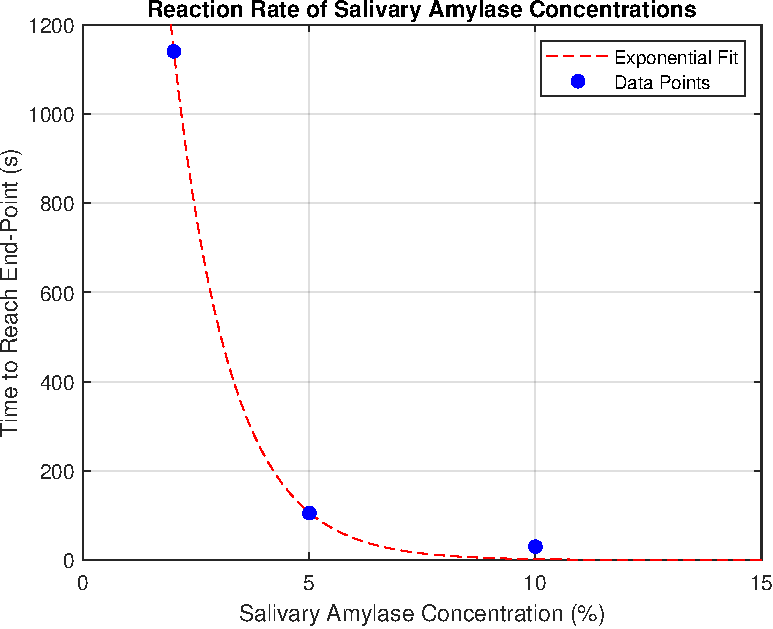
\includegraphics[width = 0.75\linewidth]{sa_curve.pdf}}
            \caption{Exponential Fit of Salivary Amylase Concentration (\%) vs. Time Required to Reach the End-Point (s).}\label{sa_curve}
        \end{figure}

        Table~\ref{p_results} shows the contents of each solution during the phosphorylase activity as well as the expected and observed results of iodine testing on each solution. The observations are the end results after iodine testing on each solution for 18 minutes in 3 minute intervals.
        \begin{table}[H]
            \caption{Phosphorylase Solution Contents and Results of Iodine Testing}
            \centering
            \begin{tabular}{@{}cccccccccc@{}}
                \toprule
                \multirow{2}{*}{\parbox{1.5cm}{\centering Test Tube \#}} & \multirow{2}{*}{Glucose} & \multirow{2}{*}{G1p} & \multicolumn{2}{c}{Starch} & \multirow{2}{*}{\(\text{HPO}_4^{2-}\) } & \multicolumn{2}{c}{Enzyme} & \multicolumn{2}{c}{Results} \\ 
                \cmidrule(lr){4-5} \cmidrule(lr){7-8} \cmidrule(lr){9-10} 
                &  &  & Primer & Excess &  & Active & Boiled & Expected & Observed \\ 
                \midrule
                1 & \blacksquare{} & \Square{} & \blacksquare{} & \Square{} & \Square{} & \blacksquare{} & \Square{} & \(-\) & \(-\) \\
                2 & \Square{} & \blacksquare{} & \blacksquare{} & \Square{} & \Square{} & \blacksquare{} & \Square{} & \(+\) & \(+\) \\
                3 & \Square{} & \blacksquare{} & \Square{} & \Square{} & \Square{} & \blacksquare{} & \Square{} & \(-\) & \(+\) \\
                4 & \Square{} & \blacksquare{} & \blacksquare{} & \Square{} & \Square{} & \Square{} & \blacksquare{} & \(-\) & \(-\) \\
                5 & \Square{} & \blacksquare{} & \blacksquare{} & \Square{} & \blacksquare{} & \blacksquare{} & \Square{} & \(-\) & \(-\) \\
                6 & \Square{} & \Square{} & \Square{} & \blacksquare{} & \blacksquare{} & \blacksquare{} & \Square{} & \(-\) & \(+\) \\
                7 & \Square{} & \Square{} & \Square{} & \blacksquare{} & \blacksquare{} & \Square{} & \blacksquare{} & \(+\) & \(+\) \\
                \bottomrule
            \end{tabular}\label{p_results}
        \end{table}

    \section*{Discussion}
        The results of the iodine and Benedict's tests in Table~\ref{sa_ib} align with expectations. 
        No reducing sugars are present in any of the solutions, confirming the absence of reducing sugars in salivary amylase solutions. 
        The starch suspension solution, as anticipated, tested positive for starch.

        The results of the salivary amylase interval test (Table~\ref{sa_interval}) also match expected results. 
        The negative iodine test end-point time decreased with increasing salivary amylase concentration, indicating accelerated starch hydrolysis. 
        The positive Benedict's test results for the solutions that reached the end-point in time confirm that the salivary amylase produced maltose, a reducing sugar, as a product of hydrolysing starch in the solution.
        
        The exponential fit of salivary amylase concentration vs.\ time (Figure~\ref{sa_curve}) illustrated a clear trend. 
        As salivary amylase concentration increased, the time required to reach the end-point decreased exponentially, in accordance with the expected enzymatic kinetics, specifically an exponential decay model. 
        Higher enzyme concentrations lead to more rapid substrate hydrolysis~\parencite{Wang2013}.
        
        The outcomes of the phosphorylase reactions (Table~\ref{p_results}) revealed varied results based on the presence or absence of specific components.
        
        The solutions in test tubes 2 and 5 had all the reactants for starch synthesis. 
        However, I predicted that only the solution in test tube 2 will undergo starch synthesis, as the solution in test tube 5 contained phosphoric acid as well, a product of starch synthesis. 
        This would put the system out of the proper concentration gradient required for starch synthesis to take place during the given time. 
        The observed results matched this prediction, with the solution in test tube 2 testing positive for starch.
        
        The solution in test tubes 6 and 7 both had excess starch. 
        Out of the two, I expected only the solution in test tube 7 to test positive for starch, as the solution in test tube 6 had all the reactants plus active enzyme for the breakdown of starch through phosphorolysis. 
        However, it was observed that both solutions did not undergo phosphorolysis, as both still tested positive for starch at the end of the given time. 
        This may indicate that the concentration gradient was not in the proper condition for the enzymatic reaction to happen fast enough.
        
        An unexpected result from the phosphorylase activity was observed in test tube 3, which had no primer or excess starch in solution. 
        Contrary to predictions, this solution tested positive for starch. 
        This discrepancy suggests possible contamination during the experiment from other solutions containing starch.

    \printbibliography{}
\end{document}